\documentclass[10pt,a4paper,titlepage]{report}
\usepackage[utf8]{inputenc}
\usepackage{amsmath}
\usepackage{graphicx}
\usepackage{amsfonts}
\usepackage{amssymb}
\usepackage[toc,page]{appendix}
\usepackage[left=2cm,right=2cm,top=2cm,bottom=2cm]{geometry}
\author{Martijn Verkleij (s1466895)}
\title{Homework Series 2}


\begin{document}
\maketitle

\chapter{Control Flow Graphs}

\section{Control Flow Graph}
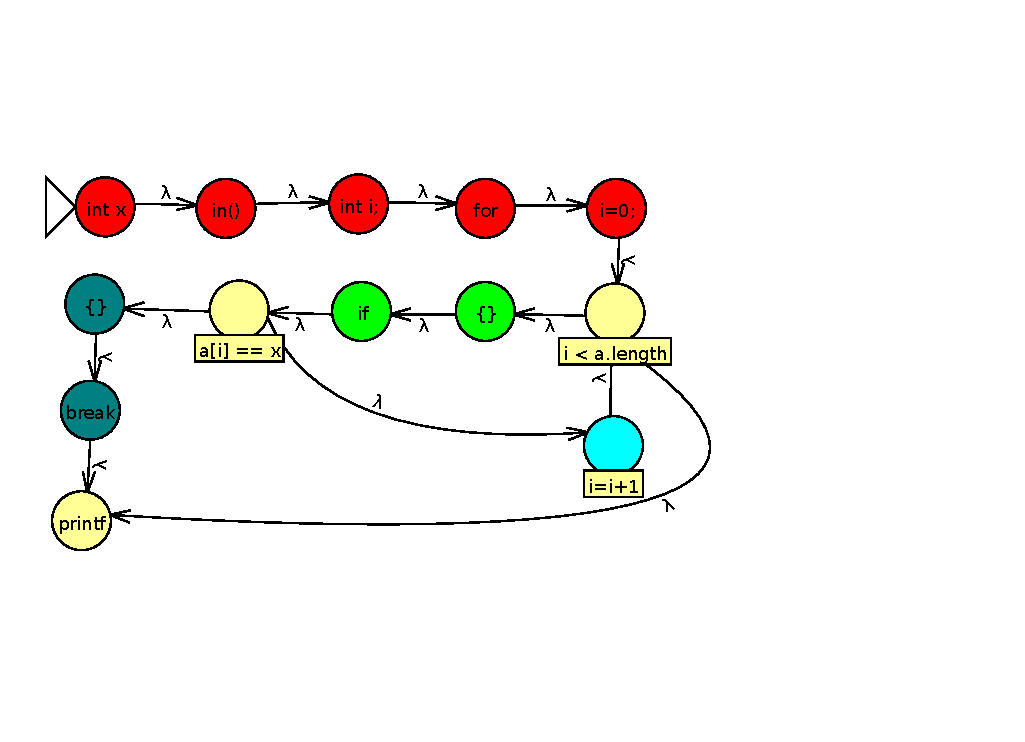
\includegraphics[width=\textwidth]{q2_1/q1_1.eps} 

\section{Control Flow Graph Uitgebreid}
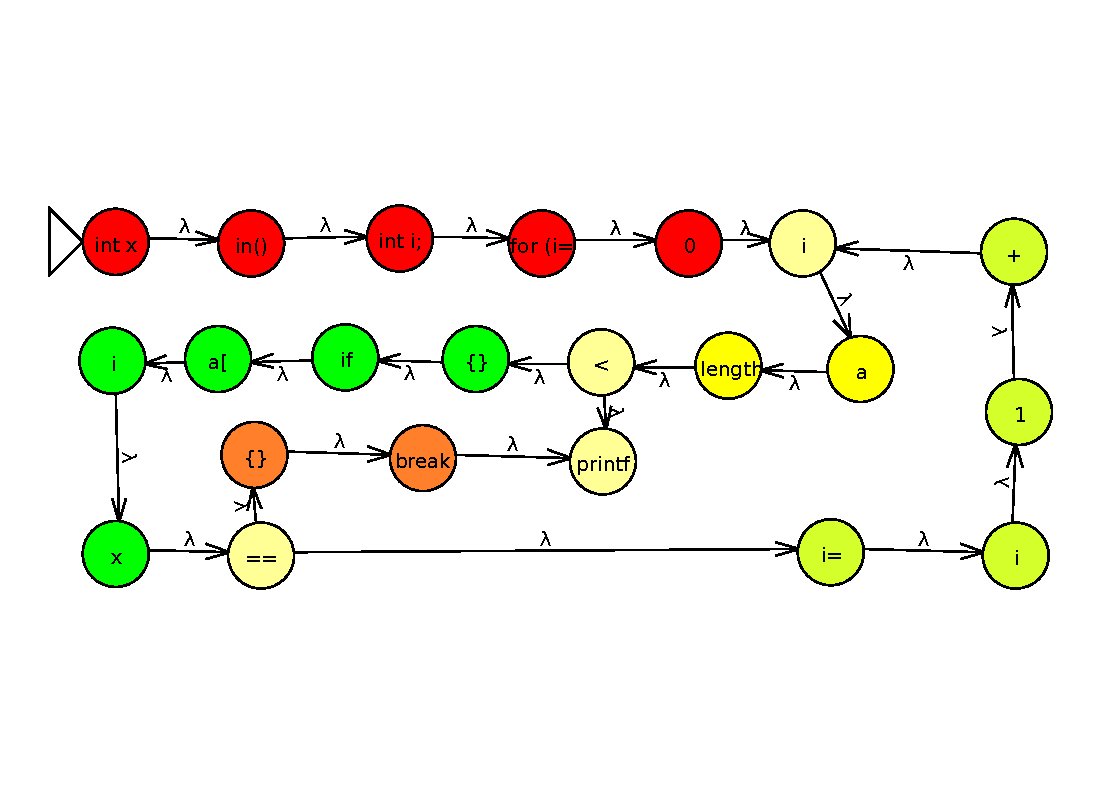
\includegraphics[width=\textwidth]{q2_1/q1_2.eps}

\section{Vergelijking}
De twee CFG's hebben op het aantal nodes na dezelfde structuur. het aantal basic blocks is bijvoorbeeld hetzelfde gebleven. Dit betekent dat de twee CFG's dezelfde gereduceerde CFG zullen opleveren. Omdat daarin alleen de basic blocks van een programma voorkomen, en deze grotere CFG's enkel uiteenzettingen van de basic blocks bevatten, zal dit ook gelden voor andere programma's.

\chapter{ILOC to CFG}
Een incomplete implementatie kan gevonden worden in \verb|s1466895/q2_2/Iloc2CFG.java|. Deze is niet in werkende staat.

\chapter{CalcCompiler}
Doel van de opgave was het maken van een TreeVisitor die een gegeven expressie omzet naar een ILOC programma dat beschikt over twee registers en een stack. Deze opgave is meegeleverd in de broncode. De tests zijn als bijlage toegevoegd.

\chapter{Activation Records}
De opgave vraagt om een representatie van de stack met de activation records. deze volgen hieronder, twee subopgaven per keer.
\section{1+2}
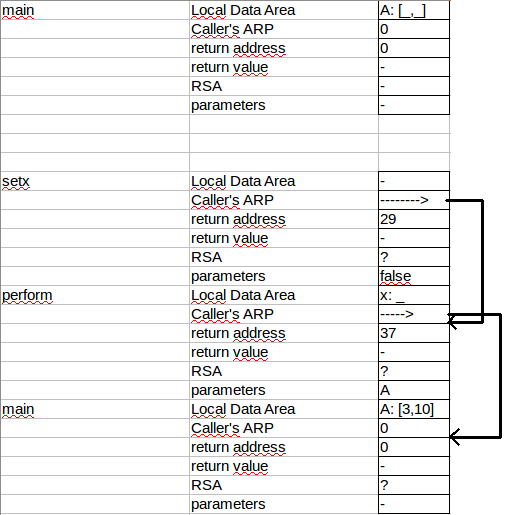
\includegraphics[width=\textwidth]{q2_4/1+2.png}
\section{3+4}
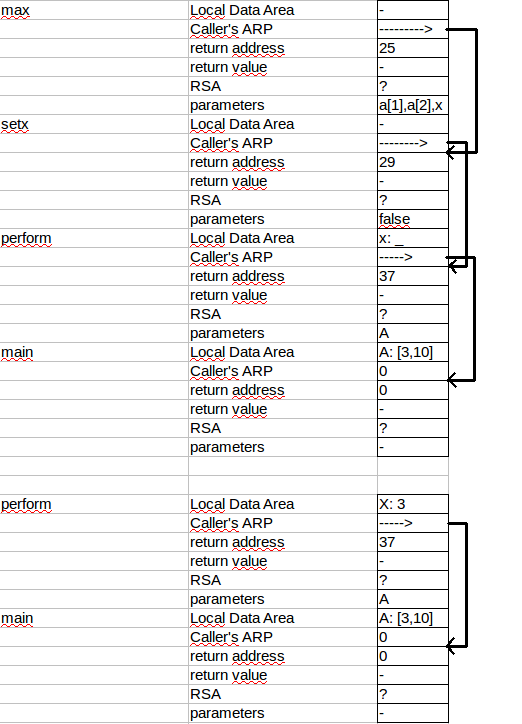
\includegraphics[width=\textwidth]{q2_4/3+4.png}

\chapter{Convert}
Het bestand \verb|s1466895/q2_5/convert.iloc| bevat een ILOC-implementatie, die in uitvoer gelijk is aan het java-programma. Het maakt gebruik van de stack voor het recursief doorgeven van de variabelen, net als in opgave \verb|6-CC.1|. De ILOC-code kan uitgevoerd worden met \verb|s1466895/q2_5/ConvertTest.java|.


\begin{appendices}
\chapter{Testresultaten opgave 3}
\section{$1+-3*4$}
\texttt{$
Processing 1+-3*4
\\Outcome: -11
\\loadI   1       => r_1 
\\push    r_1            
\\loadI   3       => r_1 
\\push    r_1            
\\pop             => r_1 
\\rsubI   r_1,0   => r_2 
\\push    r_2            
\\loadI   4       => r_1 
\\push    r_1            
\\pop             => r_1 
\\pop             => r_2 
\\mult    r_1,r_2 => r_2 
\\push    r_2            
\\pop             => r_1 
\\pop             => r_2 
\\add     r_1,r_2 => r_2 
\\push    r_2            
\\pop             => r_1 
\\out     "Outcome: ",r_1
$}
\section{$1+-(3*4)$}
\texttt{$
Processing 1+-(3*4)\\Outcome: -11
\\loadI 1 => r_1 
\\push r_1            
\\loadI 3 => r_1 
\\push r_1            
\\loadI 4 => r_1 
\\push r_1            
\\pop => r_1 
\\pop => r_2 
\\mult r_1,r_2 => r_2 
\\push r_2            
\\pop => r_1 
\\rsubI r_1,0 => r_2 
\\push r_2            
\\pop => r_1 
\\pop => r_2 
\\add r_1,r_2 => r_2 
\\push r_2            
\\pop => r_1 
\\out "Outcome: ",r_1 
$}
\section{$(1+-3)*4)$}
\texttt{$
Processing (1+-3)*4
\\Outcome: -8
\\loadI   1       => r_1 
\\push    r_1            
\\loadI   3       => r_1 
\\push    r_1            
\\pop             => r_1 
\\rsubI   r_1,0   => r_2 
\\push    r_2            
\\pop             => r_1 
\\pop             => r_2 
\\add     r_1,r_2 => r_2 
\\push    r_2            
\\loadI   4       => r_1 
\\push    r_1            
\\pop             => r_1 
\\pop             => r_2 
\\mult    r_1,r_2 => r_2 
\\push    r_2            
\\pop             => r_1 
\\out     "Outcome: ",r_1
$}

\section{$--56+(1+-3)*4$}
\texttt{$
Processing --56+(1+-3)*4
\\Outcome: 48
\\loadI   56      => r_1 
\\push    r_1            
\\pop             => r_1 
\\rsubI   r_1,0   => r_2 
\\push    r_2            
\\pop             => r_1 
\\rsubI   r_1,0   => r_2 
\\push    r_2            
\\loadI   1       => r_1 
\\push    r_1            
\\loadI   3       => r_1 
\\push    r_1            
\\pop             => r_1 
\\rsubI   r_1,0   => r_2 
\\push    r_2            
\\pop             => r_1 
\\pop             => r_2 
\\add     r_1,r_2 => r_2 
\\push    r_2            
\\loadI   4       => r_1 
\\push    r_1            
\\pop             => r_1 
\\pop             => r_2 
\\mult    r_1,r_2 => r_2 
\\push    r_2            
\\pop             => r_1 
\\pop             => r_2 
\\add     r_1,r_2 => r_2 
\\push    r_2            
\\pop             => r_1 
\\out     "Outcome: ",r_1 
$}

\end{appendices}


\end{document}